\scanpage{13}
\mspage{2}

\figure{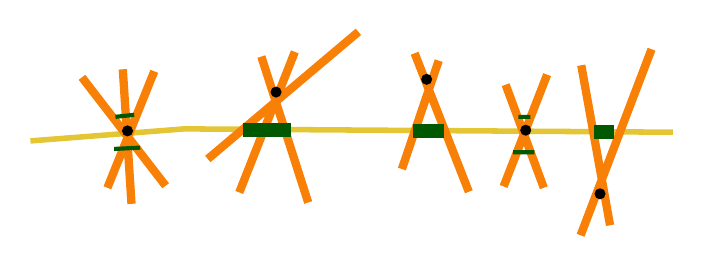
\begin{tikzpicture}[x=.85cm,y=.85cm]
\draw[yellow!55!brown,line width=2pt] (-.6,-.08)--(1.7,.10)--(9,.05);
\draw[orange!90!brown,line width=3pt] (.55,-.78)--(1.25,.96) (.17,.87)--(1.42,-.75) (.78,.99)--(.91,-1.02);
\draw[orange!90!brown,line width=3pt] (2.05,-.35)--(4.3,1.55) (2.52,-.85)--(3.35,1.25) (2.85,1.18)--(3.55,-1.00);
\draw[orange!90!brown,line width=3pt] (4.95,-.50)--(5.50,1.12) (5.14,1.23)--(5.95,-.84);
\draw[orange!90!brown,line width=3pt] (6.47,-.76)--(7.12,.91) (6.5,.76)--(7.07,-.78);
\draw[orange!90!brown,line width=3pt] (7.63,1.05)--(8.06,-1.34) (7.62,-1.49)--(8.68,1.29);
\draw[black!65!green,line width=5pt] (2.57,.08)--(3.29,.08) (5.11,.07)--(5.58,.07) (7.82,.05)--(8.12,.05);
\draw[black!65!green,line width=1.5pt] (.67,.28)--(.95,.31) (.65,-.20)--(1.04,-.18) (6.69,.28)--(6.87,.28) (6.61,-.25)--(6.93,-.25);
\foreach \x/\y in {.85/.07,3.07/.65,5.32/.84,6.80/.08,7.91/-.87}{\fill (\x,\y) circle(2pt);}
\end{tikzpicture}}

Chaque élément de $\operatorname{Sp}_0(D)$ définit un arc \deleted{(fermé)} sur $\widetilde D$, ces arcs étant mutuellement disjoints; chaque pt de $\operatorname{Gen}_0(D)$ définit un \deleted{\unsure{élément}}\inserted{pt} de $\widetilde D$, ces pt étant tous différents et non contenus dans les \deleted{\unsure{alternativement}} arcs précédents. Il en résulte une \uline{structure polygonale} sur l'ens $\operatorname{Sp}_0(D)\amalg\operatorname{Gen}_0(D)$, qui \deleted{\unsure{se}} s'identifie aussi à l'ens des arcs issus du sommet $D$ du graphe $\Gamma(\underline\Sigma)$. \deleted{Ce polygone a au moins}\inserted{Cet ens. a au moins} trois éléments je crois. \deleted{C'est} Il y en a \unsure{en} au moins quatre bien sûr si $\operatorname{card}S\cap D\geq2$, donc il suffit de regarder les cas $\operatorname{card}S\cap D\in\{0,1\}$. Dans le cas d'une $D$ ``stable'' i.e. $\operatorname{card}S\cap D=0$, il faut prouver qu'il y a au moins \deleted{deux} trois triangles de spécialisation, \unsure{disons}, dans le cas \deleted{de} $\operatorname{card}S\cap D=1$ \deleted{il f} (cas sous-stable) il faut montrer qu'il y en a au moins un.

\figure{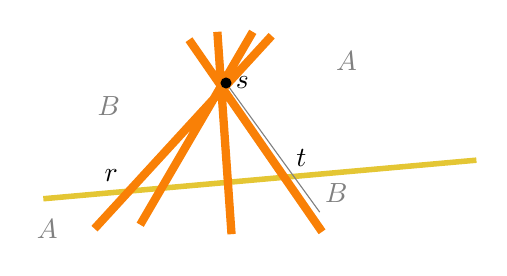
\begin{tikzpicture}[x=1cm,y=1cm]
\draw[yellow!55!brown,line width=2pt] (-.7,.13)--(4.8,.62);
\draw[gray,thin] (.63,-.10)--(1.62,1.6)--(2.81,-.04);
\draw[orange!90!brown,line width=3pt] (-.05,-.25)--(2.20,2.20) (.53,-.20)--(1.96,2.25) (1.69,-.32)--(1.51,2.25) (2.84,-.29)--(1.15,2.15);
\fill (1.62,1.6) circle(2pt);\node[right] at (1.62,1.6){$s$};
\node[above left] at (.37,.23){$r$};\node[above right] at (2.39,.42){$t$};
\node[gray] at (-.65,-.25){$A$};\node[gray] at (.13,1.31){$B$};\node[gray] at (3.15,1.88){$A$};\node[gray] at (3.02,.20){$B$};
\end{tikzpicture}}

a) Cas $D$ stable. On sait que $D$ forme au moins trois triangles (i.e. il y a au moins $3$ triangles de $\Sigma'$ adjacents à $D$), considérons en un. Il est immédiat qu'il est contenu dans un unique triangle de spécialisation $T$. Considérons les deux ``grands triangles'' \deleted{définis} $A$ et $B$ (cf figure) définis par $T$, \deleted{\unsure{adjacents}} adjacents le long de l'arc extérieur $(t,r)$ sur $D$, et \deleted{\unsure{ayant comme côtés}}\inserted{incidents resp. à $(s,r)$ et à $(s,t)$}. Dans chacun, il y a un triangle au moins de $\unsure{\widetilde\Sigma|\Sigma'}$, adjacent à $D$. Chacun de ces triangles est contenu à son tour dans un unique triangle de spécialisation, $T'$ resp. $T''$. D'où les trois triangles cherchés $T,T',T''$.

b) Cas $D$ sous-stable. \inserted{Soit $a$ le sommet de $\Sigma$ qui est \unsure{sur $D$}.} Il y a au moins \uline{trois} triangles \deleted{de} de $\Sigma'$ adj. à $D$, \deleted{\unsure{pour montrer}} \deleted{\unsure{on doit les considérer}}\inserted{Considérons une générisation $D'$ de $D$}, sur laquelle on ``éclate'' un arc $bc$ (cf. figure), \unsure{l'un|pour} des triangles de

\margin{12}
